\documentclass[aspectratio=169,usenames,dvipsnames]{beamer}


\usetheme{default}  % You can choose any other theme you prefer

\title{07 - Algoritmos}
\subtitle{Grafos - DFS e BFS}
\author{Mateus Oliveira de Figueiredo}
\date{}

\usepackage{tikz}
\usetikzlibrary{matrix}
\usepackage{multicol}
\usepackage{algorithm}
\usepackage{algpseudocode}
\usepackage{xcolor}
\usepackage[utf8]{inputenc}
\usepackage[portuguese]{babel}
\usepackage{amsmath} % for "pmatrix" environment  
\usepackage{pgffor} 

\usepackage{pgfplots}
\DeclareUnicodeCharacter{2212}{−}
\usepgfplotslibrary{groupplots,dateplot}
\usetikzlibrary{patterns,shapes.arrows, positioning}
\pgfplotsset{compat=newest}

\begin{document}

\begin{frame}
\titlepage
\end{frame}

\begin{frame}
\frametitle{Grafos}
\vfill
\begin{itemize}
  \item  Algoritmos:
  \begin{itemize}
    \item BFS: Busca em Largura (fila)
    \item DFS: Busca em Profundidade (pilha)
  \end{itemize}
  \item Dados da ANAC 
  \item Utilizada biblioteca Geopandas (plot)
\end{itemize}
\vfill
\end{frame}

\begin{frame}
  \frametitle{Questão 01 - Item A e B}
  \begin{columns}
    \begin{column}{0.3\textwidth}
      \begin{itemize}
        \item Recife e Natal estão conectados
        \item Recife e Paris não estão conectados
      \end{itemize}
    \end{column}
    \begin{column}{0.7\textwidth}
      \begin{figure}
        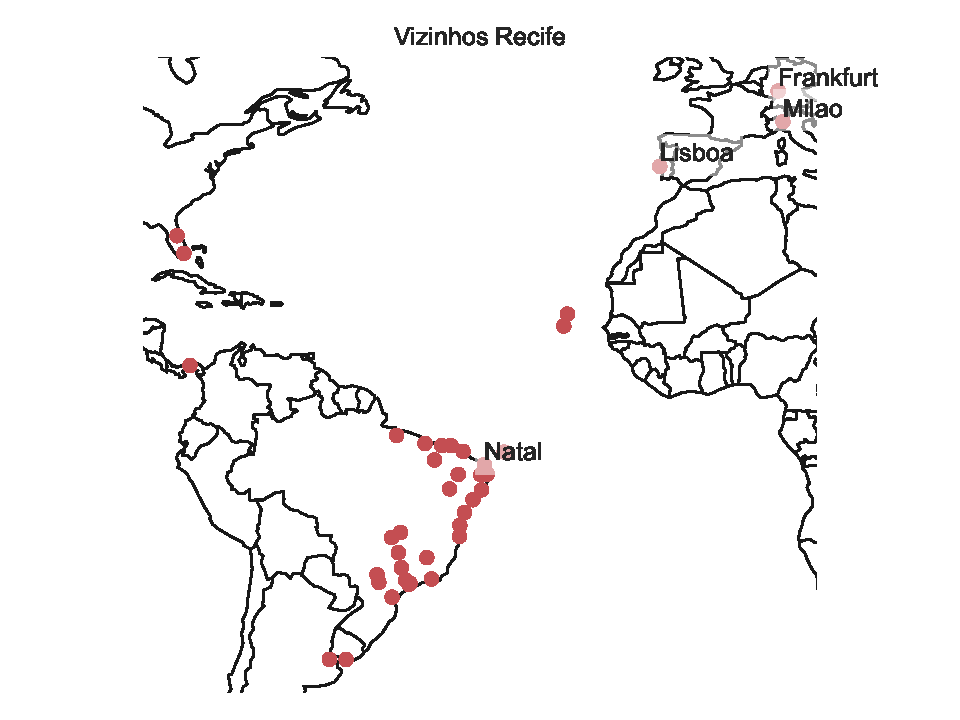
\includegraphics[width=0.9\textwidth]{figs/vizinhos_recife.pdf}
      \end{figure}
    \end{column}
  \end{columns}
\end{frame}

\begin{frame}
  \frametitle{Questão 01 - Item C}
  Dois aeroportos: Santos Dumont e Galeão
  
  \begin{figure}
    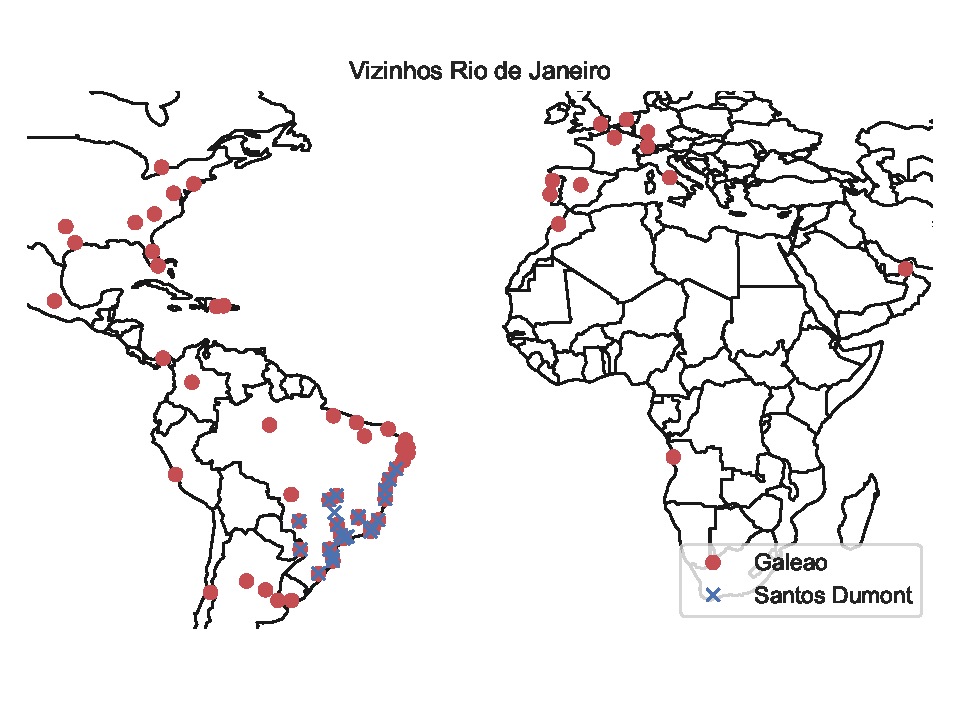
\includegraphics[width=0.7\textwidth]{figs/vizinhos_rio_de_janeiro.pdf}
  \end{figure}

  Total de 66 cidades alcançadas.
\end{frame}

\begin{frame}
  \frametitle{Questão 01 - Item D}

  \begin{tabular}{|c|c|c|}
    \hline
    Cidade & Aeroporto & \#Vizinhos \\
    \hline
    Guarulhos & Guarulhos - Governador Andre Franco Montoro & 106 \\
    \hline
    Campinas & Viracopos & 72 \\
    \hline
    Rio De Janeiro & Aeroporto Internacional Do Rio De Janeiro/Galeao & 64 \\
    \hline
    Brasilia & Presidente Juscelino Kubitschek & 59 \\
    \hline
    Confins & Tancredo Neves & 55 \\
    \hline
    Recife & Guararapes - Gilberto Freyre & 39 \\
    \hline
    Sao Paulo & Congonhas & 37 \\
    \hline
    Salvador & Deputado Luis Eduardo Magalhaes & 32 \\
    \hline
    Porto Alegre & Salgado Filho & 31 \\
    \hline
    Manaus & Eduardo Gomes & 30 \\
    \hline
  \end{tabular}

\end{frame}

\begin{frame}
  \frametitle{Questão 01 - Item D}
  \begin{center}
    \begin{tabular}{|c|c|}
    \hline
    Cidade & \#Vizinhos \\
    \hline
    Guarulhos & 106 \\
    \hline
    Campinas & 72 \\
    \hline
    Rio De Janeiro & 66 \\
    \hline
    Brasilia & 59 \\
    \hline
    Confins & 55 \\
    \hline
    Recife & 39 \\
    \hline
    Sao Paulo & 37 \\
    \hline
    Salvador & 32 \\
    \hline
    Porto Alegre & 31 \\
    \hline
    Manaus & 30 \\
    \hline
    \end{tabular}
  \end{center}
\end{frame}


\foreach \i in {001, 036, 189} {
\begin{frame} {Questão 03 - Item A}

  \begin{figure}
    \includegraphics[width=0.7\textwidth]{figs/paths/path_\i.pdf}
  \end{figure}
  
\end{frame}
}

\begin{frame} {Questão 03 - Item B}

  \begin{figure}
    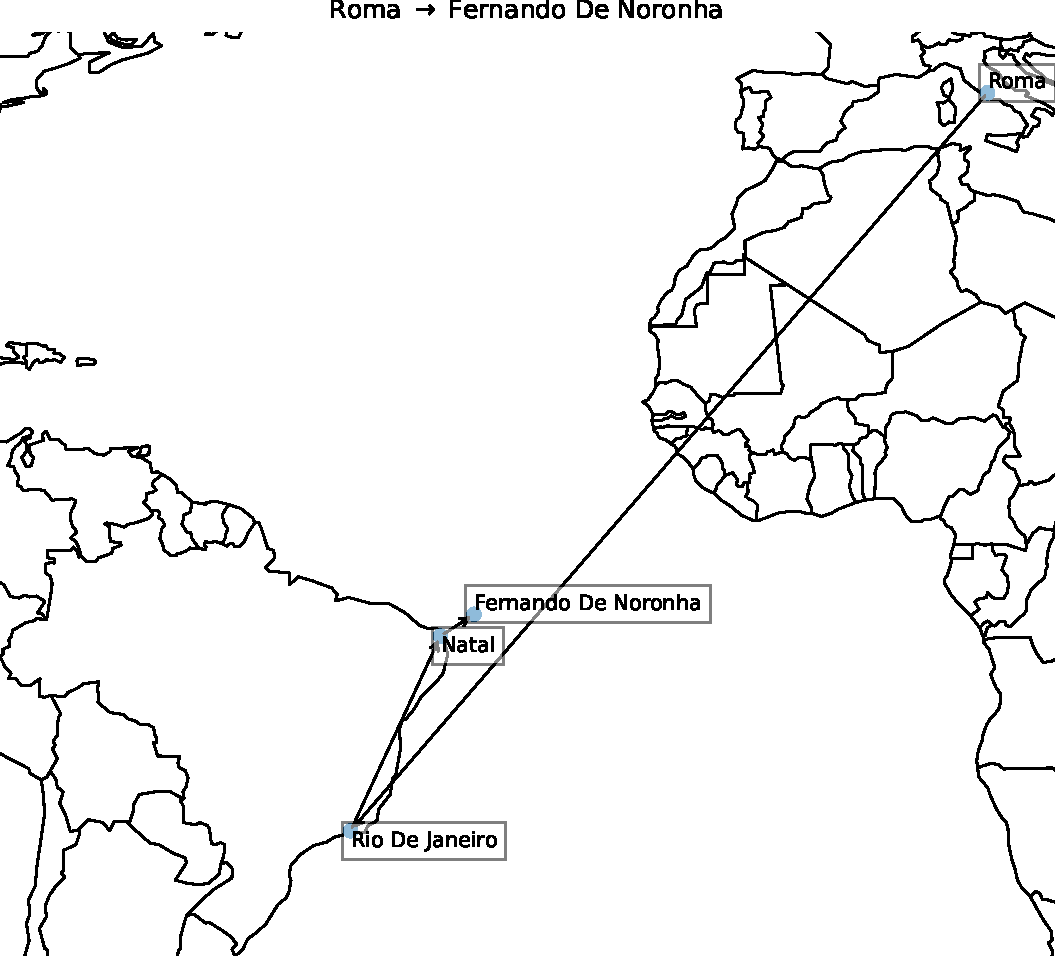
\includegraphics[width=0.7\textwidth]{figs/roma_fernando_noronha_names.pdf}
  \end{figure}

  $ Roma \rightarrow Rio de Janeiro \rightarrow Natal  \rightarrow Fernando de Noronha $
  
\end{frame}

\begin{frame}{ Questão 3 - Item C - Grafo Completo }
  \begin{columns}
    \begin{column}{0.5\textwidth}
      \begin{itemize}
        \item $m = \frac{n(n-1)}{2}$
        \item O(n + m) = O($n ^ 2$)
      \end{itemize}
    \end{column}
    \begin{column}{0.5\textwidth}
      \begin{figure}
        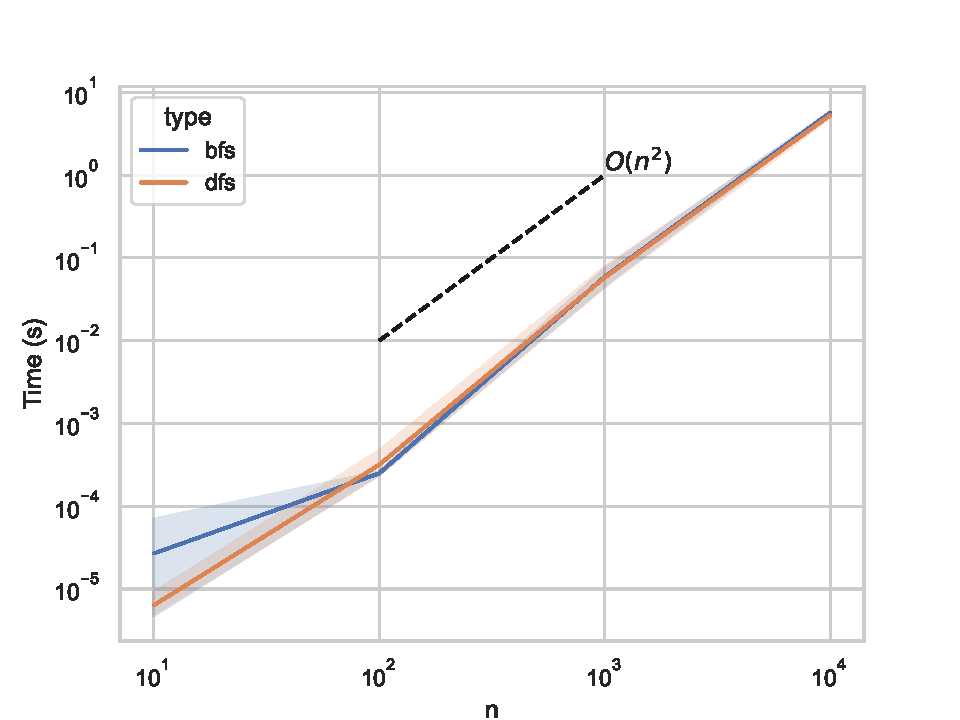
\includegraphics[width=0.9\textwidth]{figs/time_complete_graph.pdf}
        \caption{Grafo Completo}
      \end{figure}
    \end{column}
  \end{columns}
\end{frame}

\begin{frame}{ Questão 3 - Item C - Grafo Aleatório }
  \begin{columns}
    \begin{column}{0.5\textwidth}
      \begin{itemize}
        \item $m = O(\sqrt{n})$
        \item $ O(n + m) = O(n + \sqrt{n}) = O(n) $
      \end{itemize}
    \end{column}
    \begin{column}{0.5\textwidth}
      \begin{figure}
        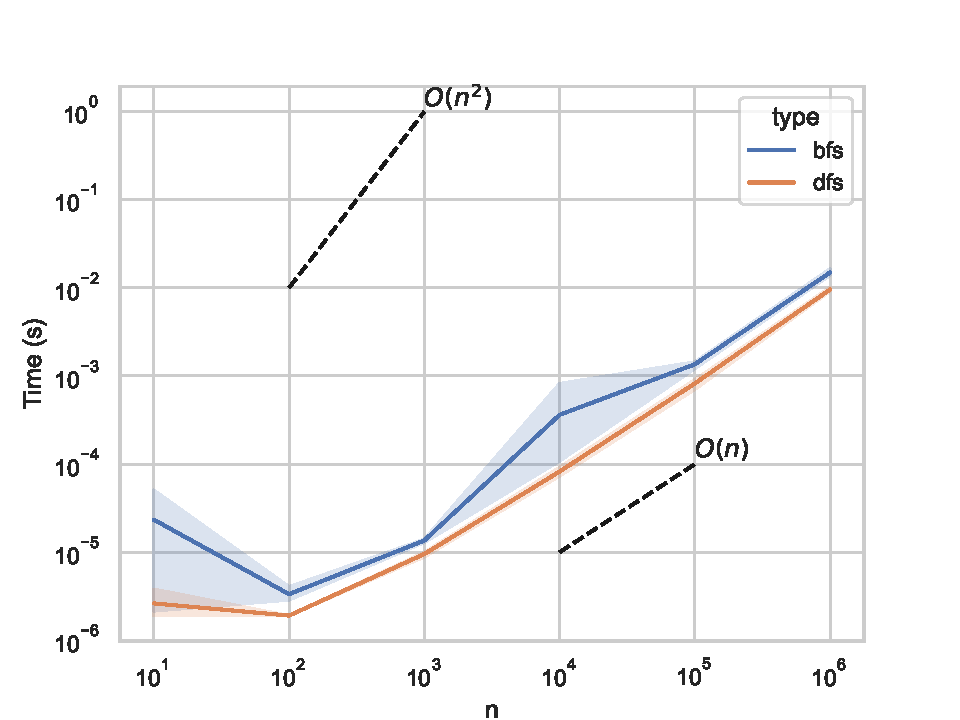
\includegraphics[width=0.9\textwidth]{figs/time_sqrt_graph.pdf}
        \caption{Grafo Aleatório}
      \end{figure}
    \end{column}
  \end{columns}
\end{frame}

\end{document}